\documentclass[11pt]{article}
\usepackage{tikz}
\usepackage{pgffor}
\usetikzlibrary{shapes}
\usetikzlibrary{arrows}
\usetikzlibrary{trees}
\usetikzlibrary{patterns}

\begin{document}

\begin{figure}
\begin{center}

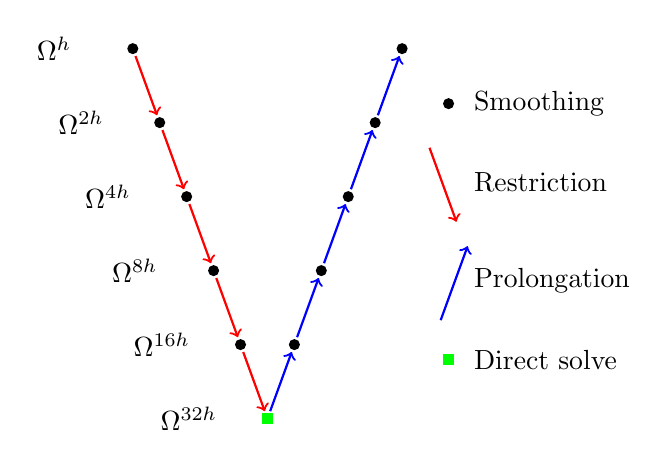
\begin{tikzpicture}[scale=1.0]

 \path (0,0) coordinate (C);
 \path (110:1) coordinate (L1l);
  \path (70:1) coordinate (L1r);
  \path (110:2) coordinate (L2l);
  \path (70:2) coordinate (L2r);    
  \path (110:3) coordinate (L3l);
  \path (70:3) coordinate (L3r);
  \path (110:4) coordinate (L4l);
  \path (70:4) coordinate (L4r);
  \path (110:5) coordinate (L5l);
  \path (70:5) coordinate (L5r);
         
  \foreach \i in {L1l,L2l,L3l,L4l,L5l,L1r,L2r,L3r,L4r,L5r}
  {
     \fill[black] (\i) circle (2pt);
  }
    
 \fill[green] (C) ++(-2pt, -2pt) rectangle +(4pt, 4pt);
    
 \draw[<-, thick, red] (C) ++(110:0.1) -- ++(110:0.8);
 \draw[<-, thick, red] (L1l) ++(110:0.1) -- ++(110:0.8);
 \draw[<-, thick, red] (L2l) ++(110:0.1) -- ++(110:0.8);
 \draw[<-, thick, red] (L3l) ++(110:0.1) -- ++(110:0.8); 
 \draw[<-, thick, red] (L4l) ++(110:0.1) -- ++(110:0.8);
 							
 \draw[->, thick, blue] (C) ++(70:0.1) -- ++(70:0.8); 
 \draw[->, thick, blue] (L1r) ++(70:0.1) -- ++(70:0.8); 
 \draw[->, thick, blue] (L2r) ++(70:0.1) -- ++(70:0.8); 
 \draw[->, thick, blue] (L3r) ++(70:0.1) -- ++(70:0.8); 
 \draw[->, thick, blue] (L4r) ++(70:0.1) -- ++(70:0.8); 
 
 \draw (C) ++(-1,0) node {$\Omega^{32h}$};
 \draw (L1l) ++(-1,0) node {$\Omega^{16h}$};							
 \draw (L2l) ++(-1,0) node {$\Omega^{8h}$};							
 \draw (L3l) ++(-1,0) node {$\Omega^{4h}$};							
 \draw (L4l) ++(-1,0) node {$\Omega^{2h}$};							
 \draw (L5l) ++(-1,0) node {$\Omega^{h}$};
  
 \fill[black] (2.3, 4) circle (2pt);
 \draw[right] (2.5, 4) node {Smoothing};      

 \draw[<-, thick, red] (2.4, 2.5) -- +(110:1);
 \draw[right] (2.5, 3) node {Restriction};

 \draw[->, thick, blue] (2.2, 1.25) -- +(70:1);
 \draw[right] (2.5, 1.75) node {Prolongation};
    
 \fill[green] (2.3, 0.75) ++(-2pt, -2pt) rectangle +(4pt, 4pt);
 \draw[right] (2.5, 0.75) node {Direct solve};

\end{tikzpicture} 

\end{center}
\end{figure}

\end{document}
			